\section{Emission Rules}
Ergo emission properties are defined by the following parameters in a monetary section of the config:

\begin{itemize}
    \item{\em fixedRatePeriod } - number of blocks since the genesis block the reward will not change.
    For mainnet it equals to 525600 that corresponds to 2 years (assuming 2 minutes block interval)
    \item{\em fixedRate } - number of coins issued every block during the $fixedRatePeriod$.
    For mainnet it equals to 7500000000 (75 coins with 8 digits).
    \item{\em epochLength } - number of blocks between reward reduction after the $fixedRatePeriod$.
    For mainnet it equals to 64800 (3 month).
    \item{\em oneEpochReduction } - number of coins reward decrease every epochs.
    For mainnet it equals to 300000000 (3 coins with 8 digits).
\end{itemize}

Thus for the first $fixedRatePeriod$ blocks miner reward will be equals to $fixedRate$ \ergo{} coins,
after $fixedRatePeriod$ block reward will be reduced for $oneEpochReduction$ coins every $epochLength$ blocks.
Mainnet parameters will lead to 8 years of coins emission with 97739925 coins total.

Taking all these concepts into consideration, Ergo's emission curve is as illustrated at Fig. \ref{fig:emission}:

\begin{figure}[H]
    \centering
    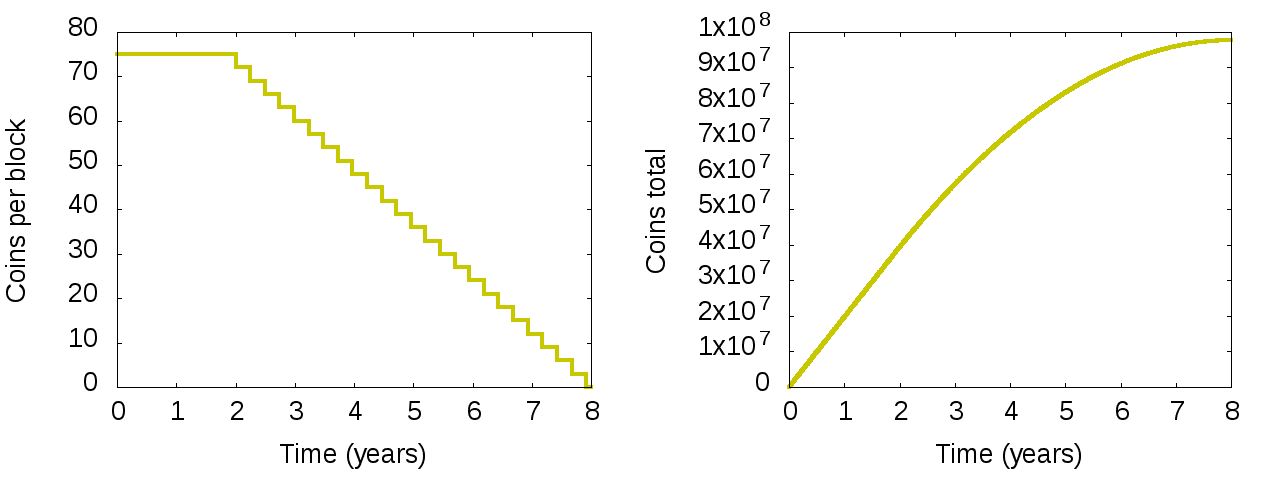
\includegraphics[width=\textwidth]{img/curve_combined.png}
    \caption{Ergo mainnet emission rules
    \label{fig:emission}}
\end{figure}


Instead of having implicit emission rules via a special type of transaction (e.g. coinbase transaction in Bitcoin),
Ergo coins emission is defined explicitly by sigma-state transactional language.
All \ergo{} coins will be created in the genesis state in an output, protected by the following script:

\begin{minted}{js}
    let epoch = 1 + ((HEIGHT - fixedRatePeriod) / epochLength)
    let out = OUTPUTS(0)
    let coinsToIssue = if(HEIGHT < fixedRatePeriod) fixedRate
    else fixedRate - (oneEpochReduction * epoch)
    let correctCoinsConsumed = coinsToIssue == (SELF.value - out.value)
    let sameScriptRule = SELF.propositionBytes == out.propositionBytes
    let heightIncreased = HEIGHT > SELF.R3[Long].value
    let heightCorrect = out.R3[Long].value == HEIGHT
    let lastCoins = SELF.value <= oneEpochReduction
    (correctCoinsConsumed && heightCorrect && heightIncreased && sameScriptRule) ||
    (heightIncreased && lastCoins)
\end{minted}

This protection script allows miner to take only a part of all coins, corresponding to current block reward.
Fist, this script calculates $coinsToIssue$ - number of coins, current miner takes to himself,
and checks, that the remaining  number of coins in the first output $out$ equals to initial
number of coins minus $coinsToIssue$.
This prevents the miner to take more coins, than defined by the emission rules.
Second, script checks that register $R3$ of $out$ contains current height and this height is greater, then height
kept in $R3$ register of spending input.
This prevents the miner to take use this output more then once per block.
Finally, it checks that $out$ have the same protecting script, preventing further miners to break emission rules.
Special case is required to stop emission - when this output contains less coins than $oneEpochReduction$,
creation of a new output is not required.
